%============================== Setting teh Document=============================================

\documentclass[aspectratio=169]{beamer}
\usepackage[italian]{babel} 
\usepackage[utf8]{inputenc} 
\usepackage[T1]{fontenc}
\usepackage{graphicx}
\usepackage{hyperref}
\usepackage{xcolor}
\usepackage{amsmath,amssymb,lmodern}
\usetheme{AnnArbor}
\usepackage{animate}

\newcommand*{\vet}{\fontfamily{qzc}\selectfont}

% in way to comment a block
\long\def\/*#1*/{}

%==========================Set the foot line========================================================
\makeatletter

\setbeamercolor*{author in head/foot}{parent=palette tertiary}
\setbeamercolor*{title in head/foot}{parent=palette secondary}
\setbeamercolor*{date in head/foot}{parent=palette primary}

\setbeamercolor*{section in head/foot}{parent=palette tertiary}
\setbeamercolor*{subsection in head/foot}{parent=palette primary}
% colors for the external link field
\setbeamercolor*{external link}{parent=palette secondary}

\defbeamertemplate*{footline}{}
{
	\leavevmode%
	\hbox{%
		\begin{beamercolorbox}[wd=.25\paperwidth,ht=2.25ex,dp=1ex,center]{author in head/foot}%
			\usebeamerfont{author in head/foot}\insertsection
		\end{beamercolorbox}%
		\begin{beamercolorbox}[wd=.25\paperwidth,ht=2.25ex,dp=1ex,center]{title in head/foot}\insertsubsection
		\end{beamercolorbox}%
		\begin{beamercolorbox}[wd=.25\paperwidth,ht=2.25ex,dp=1ex,center]{date in head/foot}%
			\usebeamerfont{date in head/foot}\insertshortdate{}\hspace*{2em}
			\insertframenumber{} / \inserttotalframenumber 
		\end{beamercolorbox}%
		% this is a new field with an external link
		\begin{beamercolorbox}[wd=.25\paperwidth,ht=2.25ex,dp=1ex,right]{external link}%
			\usebeamerfont{author in head/foot}\hyperlink{index}{indice}    \hspace*{2ex}
	\end{beamercolorbox}}%
	\vskip0pt%
}

\setbeamersize{text margin left=1em,text margin right=1em}

\makeatother



\title{Il VHF marino e le procedure di radio telefonia} 
\author{Francesco Rombaldoni\\
Alias Rombo} 
\date{}

\institute{Università degli Studi di Urbino "Carlo Bo"} 
\logo{
\includegraphics[width=15mm]{Imgs/Uni}}

\setbeamercovered{dynamic}

%===========================================Document starting===============================================
\begin{document}
	
	% Cover Page
	\begin{frame} 
		\maketitle 		
	\end{frame}
	
	% Index Page
	\begin{frame}[label = index]
		%\index{generate}
		\tableofcontents
	\end{frame}

	\section{Premessa}
	\begin{frame}
		\centering{{\textcolor{blue!80}{\huge{\textbf{Premessa}}}}}\\
	\end{frame}

	\begin{frame}{Premessa}
		%\framesubtitle{Parte 1}
		\textbf{L'obiettivo di questa relazione è di esporre il funzionamento, l'utilizzo e la manutenzione degli apparati radio ricetrasmittenti adottati per le radiocomunicazioni in ambito nautico.}\\
		\bigskip
		Per fare ciò la relazione sarà suddivisa in due parti:\\
		\begin{itemize}
			\item La prima parte verterà sulla teoria fisica di base degli apparati radio, al termine della quale si comprenderanno espressioni linguistiche del tipo: \emph{" La maggior parte delle trasmissioni nautiche sono effettuate utilizzando apparati VHF che modulano il segnale in frequenza"}.\\
			\item La seconda parte verterà invece sull'utilizzo e la manutenzione degli impianti ricetrasmittenti di bordo, riservando attenzione alle "buone pratiche" e alle procedure per una comunicazione efficace, al termine della parte si sarà in grado di stabilire una comunicazione con un'altra unità marina o con la capitaneria di porto.
		\end{itemize}
	\end{frame}

	\begin{frame}{Argomenti della relazione}
		\framesubtitle{Argomenti della prima parte}
		\textbf{Argomenti della prima parte.}
		\begin{itemize}
			\item Proprietà elettromagnetiche della corrente alternata.
			\item Periodo, frequenza, lunghezza e ampiezza d'onda.
			\item Modulazione d'ampiezza e Modulazione di frequenza.
			\item Le bande radio.
			\item La radio e l'impianto ricetrasmittente.
		\end{itemize}
	\end{frame}

	\begin{frame}{Argomenti della relazione}
		\framesubtitle{Argomenti della seconda parte}
		\textbf{Argomenti della seconda parte.}
		\begin{itemize}
			\item La banda nautica.
			\item I canali VHF.
			\item L'alfabeto internazionale. 
			\item La classificazione dei messaggi. 
			\item Trasmissione e ricezione.
		\end{itemize}
	\end{frame}

	\section{Contesto}
	\begin{frame}
		\centering{{\textcolor{blue!80}{\huge{\textbf{Contesto}}}}}\\
	\end{frame}

	\begin{frame}{Contesto}
		\framesubtitle{Parte 1}
		Per trasmettere informazioni, senza disporre di un collegamento fisico tra chi trasmette e chi riceve occorre far transitare su un mezzo non materiale.\\
		\bigskip
		\textbf{Nella trasmissione senza fili il mezzo materiale è costituito da \emph{onde radio}, ovvero da \emph{perturbazioni elettromagnetiche dello spazio}.}\\
		\bigskip
		Le onde radio possono veicolare le informazioni tra una stazione detta \emph{trasmittente} e una stazione detta \emph{ricevente}.\\
	\end{frame}

	\begin{frame}{Contesto}
		\framesubtitle{Parte 2}
			\textbf{Per trasmettere informazioni occorre:}\\
		\begin{itemize}
			\item Generare un'onda radio, detta \emph{onda portante} (quella che veicola le informazioni).
			\item Sovrapporre all'onda portante le informazioni che si desidera veicolare, l'onda che si ottiene è definita \emph{un'onda modulata}.
		\end{itemize} 
		\bigskip
		\textbf{Per ricevere informazioni occorre:}
		\begin{itemize}
			\item Captare l'onda radio trasmessa.
			\item Estrarre dall'onda modulata le informazioni, ovvero \emph{demodulare l'onda}.
		\end{itemize}
	\end{frame}

\section{Proprietà elettromagnetiche della corrente alternata}
\begin{frame}
	\centering{{\textcolor{blue!80}{\huge{\textbf{Proprietà elettromagnetiche della corrente alternata}}}}}\\
\end{frame}
	
\begin{frame}{Introduzione}
	%\framesubtitle{Proprietà elettromagnetiche della corrente alternata}
	Nel 1831 Faraday pubblica un resoconto di una serie di esperimenti nei quali, con modalità opportune, era riuscito a \emph{indurre in un circuito metallico una corrente elettrica} 
	facendo muovere un magnete rispetto al circuito.\\
	\bigskip
	Il fenomeno esaminato da Faraday sarà spiegato nel 1890 dagli studi  sulle interazioni del campo elettrico e del campo magnetico su una carica elettrica svolti da Lorentz; gli studi dimostrano infatti che se una carica elettrica è situata in un campo elettrico e in un campo magnetico sovrapposti, allora su di essa agisce una forza proporzionale: al valore della carica, dalla sua velocità e dall'intensità dei due campi. 
\end{frame}

\begin{frame}{Forza di Lorentz}
	\framesubtitle{Parte 1}
	La forza di Lorentz si ottiene a partire dalla formula per determinare la forza {\vet $\vec{F}$} prodotta da un conduttore di lunghezza {\vet $\vec{l}$} attraversato da una corrente d'intensità {\vet i} e immerso in un campo magnetico uniforme {\vet $\vec{B}$}.\\
	\medskip
	\centering{{\textcolor{red!80}{{\vet$\vec{F}$} = {\vet i $\vec{l}$} X {\vet$\vec{B}$}}}}\\
	\medskip
	\raggedright{Nella quale l'intensità della corrente {\vet i} è considerabile sulla base dell'interpretazione microscopica della corrente:}\\
	\medskip
	\centering{{\vet \textbf{i = e n S v}}}\\
	\medskip
	\raggedright{Dove: {\vet i}  rappresenta l'intensità della corrente, {\vet e} indica il valore assoluto della carica di un elettrone, {\vet n} indica il numero degli elettroni di conduzione contenuti nel conduttore \\ considerato, {\vet S} la sezione del conduttore considerato e {\vet v} la velocità degli elettroni di \\ conduzione presenti nel conduttore.}\\
\end{frame}

\begin{frame}{Forza di Lorentz}
	\framesubtitle{Parte 2}
	Sostituendo l'intesnità della corrente si ottiene:\\  
	\medskip
	\centering{{\textcolor{red!80}{{\vet$\vec{F}$} = {\vet e n S v $\vec{l}$} X {\vet$\vec{B}$}}}}\\
	\medskip
	\raggedright{Tenendo conto del fatto che il vettore {\vet $\vec{l}$} ha la stessa direzione della velocità di deriva {\vet v} e verso opposta ad essa, è possibile considerare la precedente relazione in questo modo:}\\
	\medskip
	\centering{ {{\vet$\vec{F}$}} = -{\vet e n S l $\vec{v}$} X{\vet$\vec{B}$}}\\
	\medskip
	\raggedright{Considerando che il prodotto {\vet S l} corrisponde al volume del conduttore di tratto {\vet l} immerso nel campo magnetico {\vet $\vec{B}$}, ne consegue che il prodotto  {\vet n S l} permette di conoscere il numero {\vet N} di elettroni presente nel conduttore di tratto {\vet l}.\\
	Si può quindi porre:\\}
	\centering{{{\vet$\vec{F}$}} = -{\vet e N $\vec{v}$} X {\vet$\vec{B}$}}\\
\end{frame}

\begin{frame}{Forza di Lorentz}
	\framesubtitle{Parte 3}
	La precedente espressione può essere estesa al caso più generare di una carica (positiva o negativa) di valore assoluto {\vet q} che si muove in un campo magnetico caratterizzato, nel punto dove si trova la carica in un certo istante, dal vettore {\vet $\vec{B}$}.\\
	Ovvero:\\
	\medskip
	\centering{{\textcolor{red!80}{{\vet$\vec{F}$} = {\vet q $\vec{v}$} X {\vet$\vec{B}$}}}}\\
	\medskip
	\raggedright{Siccome non si può escludere che, unitamente al campo magnetico, sia presente anche un campo elettrico {\vet$\vec{E}$}, allora se {\vet$\vec{E}$} indica il vettore del campo elettrico nel punto {\vet P} allora la carica {\vet q} sarà sempre soggetta ad una forza:}\\
	\medskip
	\centering{{\textcolor{red!80}{{\vet$\vec{F}$} = {\vet q $\vec{E}$} + {\vet q $\vec{v}$} X {\vet$\vec{B}$}}}}\\
\end{frame}

\begin{frame}{Corrente indotta dalla forza di Lorentz}
	%\framesubtitle{Proprietà elettromagnetiche della corrente alternata}
La relazione espressa dalla forza di Lorentz consente di prevedere che, quando, con modalità opportune, si muove un circuito (oppure una sua parte) in un campo magnetico, nel circuito si genera una corrente elettrica che non dipende dall'evventuale presenza di un generatore (ad esempio di tipo elettrochimico), per questo motivo la corrente elettrica prodotta è designata con il termine di \textbf{corrente indotta}.\\
\end{frame}

\begin{frame}{Corrente indotta e campo elettromotore}
	\framesubtitle{Parte 1}
	Considerando un \emph{circuito di forma quadrata}, realizzato con un buon conduttore, nel quale sia stato inserito un \emph{amperometro con lo zero centrale}, che sia in movimento (\emph{con velocità costante}) rispetto ad un \emph{campo magnetico uniforme},  in maniera tale che durante il movimento, il circuito entra ed esca dal campo magnetico.\\
	Supponendo che, il circuito si muovi da sinistra verso destra e che il campo magnetico sia posizionato a metà del percorso che il circuito deve compiere, si hanno cinque configurazioni del circuito rispetto al campo magnetico.\\
	\end{frame}

\begin{frame}{Corrente indotta e campo elettromotore}
	\framesubtitle{Parte 2}
	\begin{enumerate}
	\item Il circuito si trova al di fuori del campo magnetico, di conseguenza l'amperometro non indica alcun passaggio di corrente.
	\item Il circuito si trova parzialmente nel campo magnetico, di conseguenza l'amperometro indica la presenza di una corrente d'elettroni che si muove in senso orario. Questa cosa è possibile poiché sugli elettroni di conduzione agisce la forza di Lorentz, di conseguenza si produce una forza elettromotrice data dalla circuitazione del campo elettromotore.
	\item Il circuito si trova completamente immerso nel campo magnetico, di conseguenza nel tratto precedentemente non immerso nel campo magnetico, si  svilupperà un campo elettromotore. Tenendo presente che il fenomeno della corrente indotta è osservabile solo nei circuiti chiusi, è possibile dedurre che il campo elettromotore generato sia\\ opposto a quello della seconda configurazione, facendo in modo che la\\ circuitazione totale valga zero.
\end{enumerate}
	\end{frame}

\begin{frame}{Corrente indotta e campo elettromotore}
	\framesubtitle{Parte 3}
	\begin{enumerate}
		\setcounter{enumi}{3}
		\item Il circuito si trova parzialmente nel campo magnetico, di conseguenza l'amperometro indica la presenza di una corrente d'elettroni che si muove in senso antiorario. 
		\item Il circuito si trova completamente al di fuori del campo magnetico, di conseguenza in esso non sarà più presente alcun campo elettromotore associato alla forza di Lorentz e quindi non sarà percorso da alcuna corrente.
	\end{enumerate}
\end{frame}

\begin{frame}{Legge di Faraday}
	%\framesubtitle{Proprietà elettromagnetiche della corrente alternata}
	L'esperimento precedente oltre permettere di apprezzare l'esistenza della corrente indotta, permette di dimostrare che la genesi del campo elettromotore (il quale poi genera un flusso d'elettroni) è dipendente da una variazione del campo magnetico, infatti quando il circuito dell'esperimento si trovava completamente immerso nel campo magnetico, in esso la somma dei campi elettromotori individuati era nulla.\\
	Il fenomeno appena descritto è interpretabile utilizzando il concetto di flusso del campo magnetico:\\
	\medskip
		\centering{\emph{Quando ad un circuito si concatena una variazione $ \Delta \Phi (\vec{B})$ del flusso del campo magnetico nel tempo $\Delta${\vet t}, nel circuito si produce una corrente indotta determinata dalla presenza di una \textbf{forza elettromotrice} espressa dalla relazione seguente}}\\
	\medskip
	\centering{{\textcolor{red!80}{{\vet fem} = $\frac{\Delta \Phi (\vec{B})}{\Delta t}$}}}\\
	\end{frame}

\begin{frame}{Legge di Faraday-Lenz}
	%\framesubtitle{Proprietà elettromagnetiche della corrente alternata}
	La descrizione della forza elettromotrice indotta espressa dalla legge di Faraday è incompleta, perché in base ad essa non è possibile stabilire il verso di circolazione della corrente indotta.\\
	Faraday aveva dato delle indicazioni chiare sul modo di determinare il verso di circolazione, tuttavia Lenz nel 1834 espose delle osservazioni in grado di semplificare il procedimento proposto da Faraday.\\
	Le osservazioni che Lenz espose sono sintetizzabili in questo modo:\\
	\medskip
	\centering{\emph{La forza elettromotrice indotta in un circuito genera una corrente (detta corrente indotta) il cui effetto deve essere tale da opporsi alla causa che la produce.}}\\
	\medskip
	\raggedright{Per tenere conto della legge di Lenz, la legge di Faraday viene riscritta in questo modo:}\\
	\medskip
	\centering{{\textcolor{red!80}{{\vet fem} = -$\frac{\Delta \Phi (\vec{B})}{\Delta t}$}}}\\
	\end{frame}

\begin{frame}{Corrente autoindotta}
	\framesubtitle{Parte 1}
	Fino a questo momento la legge di Faraday-Lenz è stata usata per interpretare l'effetto che un campo magnetico variabile produce su un circuito chiuso.\\
	Ma un circuito in cui fluisce corrente è un elemento che, a sua volta,  genera un campo magnetico al quale (di conseguenza) si concatena un flusso del campo magnetico.\\
	Se quindi si fa variare l'intensità della corrente che fluisce nel circuito considerato, varierà anche il flusso del campo magnetico che si concatena ad esso. Questa condizione in base alla legge di Faraday-Lenz, determinerà nel circuito stesso la genesi di una corrente indotta.\\
	\medskip
	Trattandosi di corrente indotta dalla variazione dell'intensità della corrente che fluisce nel circuito stesso, essa viene usualmente denominata \textbf{Corrente autoindotta}.\\
	\end{frame}

\begin{frame}{Corrente autoindotta}
	\framesubtitle{Parte 2}
	L'intensità della \textbf{corrente autoindotta} è determinata dal valore della variazione nel tempo del flusso che si concatena al circuito. Ricordando che il valore del flusso autoconcatenato dipende a sua volta dalle caratteristiche geometriche del circuito e dalle caratteristiche del mezzo con cui il circuito è realizzato.\\
	\medskip
	\centering{\emph{In generale, ad ogni circuito è possibile associare una grandezza, denominata \textbf{coefficiente di autoindizione} (detto anche induttanza) che si indica con il simbolo{\vet L}, che connette il valore dell'intensità di corrente che fluisce nel circuito con il valore $\Phi(\vec{B})$ del flusso del campo magnetico autoconcatenato, secondo la relazione:}}\\
	\medskip
	\centering{{\textcolor{red!80}{$\Phi(\vec{B})$ = {\vet L i}}}}
\end{frame}

\begin{frame}{Radiazione elettromagnetica}
	\framesubtitle{Parte 1}
	In generale, nella realtà, un flusso variabile di $\vec{B}$ (o di $\vec{E}$) non genera un campo $\vec{E}$ (o un campo $\vec{B}$) anch'esso variabile; tuttavia in opportune condizioni ciò può accadere.\\
	\medskip
	Se $\vec{B}$ variasse sinusoidalmente secondo l'ecquazione:\\ 
	\smallskip
	{\textcolor{black!50}{${\vet B} = C_{1} \sin (\omega {\vet t})$}}\\
	\smallskip
	Il campo elettromotore associato alla variazione del flusso di $\vec{B}$ rispetto al tempo sarebbe del tipo:\\
	\smallskip
	{\textcolor{black!50}{${\vet E} = C_{2} \cos (\omega {\vet t})$}}\\
	\smallskip
	D'altra parte, ad un campo elettrico di questo tipo, è associato un flusso la cui variazione rispetto al tempo genererà un campo $\vec{B}$ del tipo:\\
	\smallskip
	{\textcolor{black!50}{${\vet B} = C_{3} \sin (\omega {\vet t})$}}
 	\end{frame}
 
 \begin{frame}{Radiazione elettromagnetica}
 	\framesubtitle{Parte 2}
 	Per cui si deduce che:\\
 	\medskip
 	\centering{\emph{Un campo magnetico variabile in modo opportuno concatena a sè un campo elettromotore, variabile in modo tale da concatenare a se un campo magnetico variabile... e così via.\\ In questo caso, i campi elettrico e magnetico concatenati costituiscono un ente fisico, solitamente indicato con il termine di \textbf{radiazione elettromagnetica}}}\\
 	\medskip
 	\animategraphics[loop,width=4cm]{10}{GifImage/Wavey/Wavey-}{0}{30}
 \end{frame}

\begin{frame}{Propagazione della radiazione elettromagnetica}
	\framesubtitle{Parte 1}
	In un generico punto distante {\vet x} dall'origine del sistema di riferimento, e nel generico istante {\vet t}, i valori di $\vec{E}$ e di $\vec{B}$ sono dati da:\\
	\medskip
	\centering{{\textcolor{red!80}{$E = E_{0} \sin [2 \pi (\frac{t}{T} - \frac{x}{\lambda})]$}}}\\
	\smallskip
	{\textcolor{red!80}{$ B = B_{0} \sin [2 \pi (\frac{t}{T} - \frac{x}{\lambda})]$}}\\
	\raggedright
	\medskip
	Dove: $\lambda$ indica la lunghezza d'onda della radiazione elettromagnetica e T indica il periodo.\\
	\medskip
	Come precedentemente osservato, i vettori $\vec{E}$ e $\vec{B}$ che caratterizzano una radiazione elettromagnetica, giacciono in piani perpendicolari fra loro, possedendo una direzione di vibrazione perpendicolare alla direzione di propagazione. Questa rappresentazione corrisponde al fatto che una radiazione elettromagnetica che si propaga nello spazio si comporta\\ come \emph{un'onda trasversale}.
\end{frame}

\begin{frame}{Propagazione della radiazione elettromagnetica}
	\framesubtitle{Parte 2}
	I moduli di $\vec{E}$ e $\vec{B}$ variano in funzione dell'intensità della radiazione, della distanza {\vet x} del punto considerato dalla sorgente e del tempo {\vet t}; tuttavia si può dimostrare che essi stanno fra loro sempre nel rapporto seguente:\\
	\medskip
	\centering{{\textcolor{red!80}{{\vet v} = $\frac{E}{B}$}}}\\
	\medskip
	\raggedright{dove {\vet v} indica la velocità di propagazione della radiazione.}\\
\end{frame}

\begin{frame}{Generazione delle radiazioni elettromagnetiche}
	\framesubtitle{Parte 1}
	La prima persona ad aver svolto esperimenti per lo studio della radiazione elettromagnetica è stato il fisico tedesco Hertz, che, nel 1882 fu in grado di generare radiazioni elettromagnetiche.\\
	L'apparecchiatura utilizzata da Hertz per studiare le radiazioni elettromagnetiche si può considerare come un trasformatore di differenza di potenziale, che tra due elettrodi produce una differenza di potenziale molto elevata, capace di provocare una scarica elettrica.\\ 
	\medskip
	Per verificare quindi l'ipotesi di propagazione del campo elettromagnetico, Hertz posizionò nelle vicinanze del generatore un secondo circuito con caratteristiche de tutto simili al primo, osservando se in questo secondo circuito (detto rilevatore) si manifestava un qualche effetto fisico dovuto alla scarica provocata dal generatore. Constatando che ogni qualvolta venisse prodotta una scarica fra gli elettrodi del generatore, veniva indotta una scarica\\ tra gli elettrodi del rilevatore.\\
\end{frame}

\begin{frame}{Generazione delle radiazioni elettromagnetiche}
	\framesubtitle{Parte 2}
	Il generatore di Hertz non è molto adatto come generatore di radiazioni elettromagnetiche, perché il circuito assorbe una grande quantità di energia. Una progressiva modifica del generatore di Hertz ha portato alle moderne \textbf{antenne ricetrasmittenti}.\\
	\medskip
	In esse, gruppi di cariche di segno opposto oscillano con moto armonico, generando intensi campi elettromagnetici.\\
	L'estrema schematizzazione di un'antenna è costituita da un \textbf{dipolo elettrico oscillante}.\\
	\medskip
	\centering{\emph{Si può dimostrare che a grandi distanze dal dipolo il campo elettrico $\vec{E}$ si trova sempre in piani passanti per il dipolo, e la sua intensità: è inversamente proporzionale alla distanza {\vet r} dal dipolo, è direttamente proporzionale al quadrato della frequenza {\vet f} di oscillazione del dipolo e dipende dall'angolo $\vartheta$ che la direzione considerata forma con l'asse del dipolo.}}\\
	\medskip
	\raggedright{Ricordando che l'intensità si un'onda è proporzionale al quadrato della sua ampiezza, si\\ ottiene la formula:}\\
	\centering{{\textcolor{red!80}{$I \div E^2 \div \frac{f^4 \sin^2 \vartheta}{r^2}$}}}
\end{frame}

\begin{frame}{Energia della radiazione elettromagnetica}
	\framesubtitle{Parte 1}
	A partire dal caso di un campo elettrico uniforme confinato tra due armature di un condensatore piano, è possibile determinare che un campo elettrico è sede di energia, la cui densità è data dalla seguente relazione:\\
	\smallskip
	\centering{$D_{E} = \frac{1}{2} \varepsilon_{0} E^2$}\\
	\smallskip
	\raggedright{Analogamente l'analisi di un particolare campo magnetico uniforme (come quello prodotto all'interno di un solenoide) consente di stabilire che anche un campo magnetico è sede di energia, la cui densità è data dalla relazione:}\\
	\smallskip
	\centering{$D_{B} = \frac{1}{2} \frac{B^2}{\mu_{0}}$}\\
	\smallskip
	\raggedright{La densità di energia $D_{E,B}$ associata al campo elettromagnetico della radiazione, quando i moduli dei campi sono $E$ e $B$ rispettivamente è allora data da:}\\
	\smallskip
	\centering{$D_{E,B} = D_{E} + D_{B} = \frac{1}{2} \varepsilon_{0} E^2 + \frac{1}{2} \frac{B^2}{\mu_{0}}$}
\end{frame}

\begin{frame}{Energia della radiazione elettromagnetica}
	\framesubtitle{Parte 2}
	I valori di {\vet E} e di {\vet B} che compaiono nella precedente relazione sono funzione del tempo {\vet t}\\
	\medskip
	\centering{$E = E_{max} \sin \omega t \qquad B = B_{max} \sin \omega t$}\\ 
	\medskip
	\raggedright{Per calcolare l'energia di una radiazione che attraversa una certa superficie, si deve perciò determinare il valore medio dell'espressione precedente, valutata su un periodo {\vet T} della radiazione. Con il calcolo integrale si trovano i seguenti valori medi:}\\
	\medskip
	\centering{$\frac{1}{4} \varepsilon_{0} E^2_{max} \quad \textrm{e} \quad \frac{1}{4} \frac{B^2_{max}}{\mu_{0}}$}\\
	\medskip
	\raggedright{Ricordando poi che $E_{max} = c B_{max}$ e che $c^2 = 1/(\varepsilon_{0} \mu_{0})$, si ottiene infine:}\\
	\medskip
	\centering{{\textcolor{red!80}{$\frac{\varepsilon_{0} E^2_{max}}{4} + \frac{E^2_{max}}{4c^2\mu_{0}} = \frac{\varepsilon_{0} E^2_{max}}{2}
				\qquad \frac{\varepsilon_{0} c^2 B^2_{max}}{4} + \frac{B^2_{max}}{4\mu_{0}} = \frac{B^2_{max}}{2\mu_{0}}$}}}
\end{frame}

\begin{frame}{Energia della radiazione elettromagnetica}
	\framesubtitle{Parte 3}
	Queste relazioni consentono di determinare l'energia elettromagnetica che attraversa l'unità di superficie nell'unità di tempo, ovvero la potenza della radiazione per unità di superficie, detta anche \textbf{potenza specifica} o \textbf{irraggiamento}.\\
	Tenendo conto, infatti che tale energia è quella che si può pensare contenuta in un cilindro di altezza $(c \cdot 1 s)$ e di base $1 m^2$, ottenendo: \\
	\medskip
	\centering{{\textcolor{red!80}{$I = \frac{1}{2} c \varepsilon_{0} E^2_{max} = \frac{1}{2} c \frac{B^2_{max}}{\mu_{0}}$}}}
\end{frame}

\section{Periodo, frequenza, lunghezza e ampiezza d'onda}
\begin{frame}
	\centering{{\textcolor{blue!80}{\huge{\textbf{Periodo, frequenza, lunghezza e ampiezza d'onda}}}}}\\
\end{frame}

\begin{frame}{Periodo e frequenza}
	%\framesubtitle{Periodo, frequenza, lunghezza e ampiezza d'onda}
	In fisica la frequenza di un fenomeno che si ripete identico nel tempo, viene data dal numero di ricorrenze dell'evento in una data unità di tempo.\\
	\smallskip
	Un modo per calcolare il valore della \textbf{frequenza} ({\vet f}) consiste nel fissare un intervallo di tempo chiamato \textbf{periodo} (T), nel contare il numero delle occorrenze dell'evento che si ripete nell'intervallo di tempo considerato e nel dividere quindi il risultato di questo conteggio per il periodo.\\
	In formula:\\
	\medskip
	\centering{{\textcolor{red!80}{{\vet f} = $\frac{1}{T}$}}}\\
	\medskip
	\raggedright{L'unità di misura della frequenza è chiamata \textbf{hertz} (Hz), dove 1Hz caratterizza un evento che occorre una volta in un secondo.}\\
	Quindi:\\
	\centering{1Hz = $\frac{1}{s}$}
\end{frame}

\begin{frame}{Lunghezza e ampiezza d'onda}
	\framesubtitle{Parte 1}
	\emph{Un'onda è una struttura ripetitiva tanto nello spazio che nel tempo.}\\
	\smallskip
	La \textbf{lunghezza d'onda} di un'onda periodica è la distanza tra due massimi o fra due minimi, e viene comunemente indicata con $\lambda$.\\
	\centering{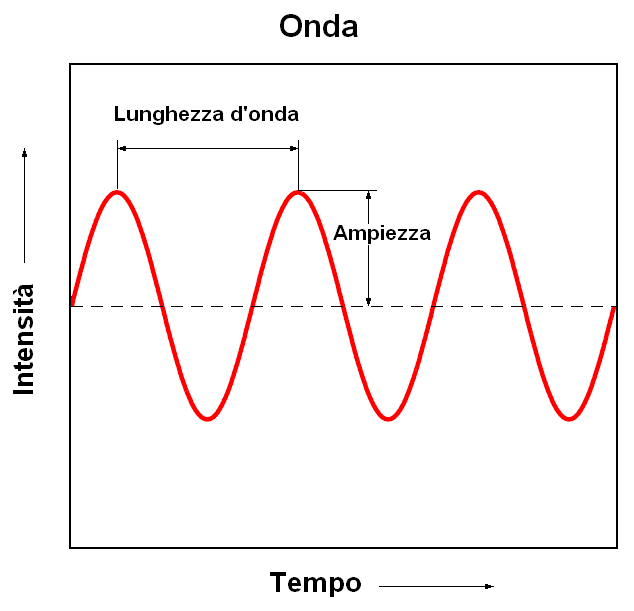
\includegraphics[scale=0.2]{Imgs/Onda}}	
\end{frame}

\begin{frame}{Lunghezza e ampiezza d'onda}
	\framesubtitle{Parte 2}
	La lunghezza d'onda $\lambda$ è definita come:\\
	\medskip
	\centering{$\lambda = \frac{{\vet v}}{{\vet f}}$}\\
	\smallskip
	\raggedright{Dove {\vet v} è la velocità di propagazione e {\vet f} la frequenza dell'onda. La velocità {\vet v} delle onde elettromagnetiche è pari alla velocità della luce (circa $3 \cdot 10^8 m\mathbin{/}s$)}.\\
	\medskip
	Per esempio, la lunghezza d'onda $\lambda$ di un segnale a 100MHz (quindi il segnale di un'onda radio) è circa:\\
	\medskip
	\centering{$\frac{3 \cdot 10^8 m\mathbin{/}s}{100 \cdot 10^6 Mh} = 3m$}\\
	\medskip
	\raggedright{In sintesi:}\\
	\emph{La \textbf{lunghezza d'onda} che viene misurata in metri, rappresenta la distanza tra i massimi ed i minimi dell'onda. Mentre il valore della sua \textbf{ampiezza} consiste nella distanza che intercorre tra il suo massimo ed il suo valore nullo.}
\end{frame}

\begin{frame}{Relazione tra lunghezza d'onda e frequenza}
	Le onde radio sono quindi delle \textbf{perturbazioni elettromagnetiche nello spazio} caratterizzate da una \textbf{lunghezza d'onda} e da una frequenza.\\
	Poiché la lunghezza d'onda e la frequenza di una radiazione sono \textbf{inversamente proporzionali}, tanto minore sarà la lunghezza d'onda, tanto maggiore sarà la frequenza.\\
	\medskip
	Per esempio:\\
	\centering
	\begin{tabular}{|c|c|c|}
		\hline
		\textbf{Banda}& \textbf{Frequenza} & \textbf{Lambda} \\
		\hline
		O M (radioamatori)& 14Mhz & 21m \\
		\hline
		C B (banda cittadina)& 27Mhz & 11m\\
		\hline
		A G (aviazione)& 118Mhz & 2,54m \\
		\hline
		Nautica VHF (marittima)& 156Mhz & 1.92m \\
		\hline
	\end{tabular}
\end{frame}

\section{Modulazione d'ampiezza e Modulazione di frequenza}
\begin{frame}
	\centering{{\textcolor{blue!80}{\huge{\textbf{Modulazione d'ampiezza e Modulazione di frequenza}}}}}\\
\end{frame}

\end{document}